\noindent To build a relativistic QFT, we start with an effective model from a \textit{classical field theory}, and make an "educated guess" to quantize the classical field theory. The desired relativistic QFT has nothing to do \textit{a priori} with the classical field theory. After quantization, the "educated guess", we take the limits of low energy, large scale, and decoherence, and check that we get back the classical field theory we started with, demonstrating whether the chosen quantization is correct or incorrect... enough, to some level of approximation.

\subsection*{Fields}

\noindent A \textit{field} is a quantity (e.g., density, spin, charge) tht is defined at every point on a manifold $\mathcal{M}$. Note that a rigorous definition of a field requires the introduction of vector bundles, of which we will not go so far. \\
We work on the Minkowski spacetime manifold $\mathcal{M} = \mathcal{M}_{1,3} = \mathbb{R}^1 \times \mathbb{R}^3$, with the field often taken to be two-times differentiable such that $\phi \in C^2(\mathcal{M}, \rho)$ and defined as a function from the manifold to some target space $\rho$
\begin{equation}
\phi : \mathcal{M} \rightarrow \rho 
\end{equation}

\noindent Some target spaces $\rho$, their associated field type, and example applications and models include

\begin{itemize}
\item $\rho = \mathbb{R}$; \textbf{scalar field}; charge density, magnetization density, Higgs boson
\item $\rho = \mathbb{R}^n$; \textbf{vector field}; electromagnetic field (actually a gauge field), pions
	\begin{figure}[H]
		\centering
		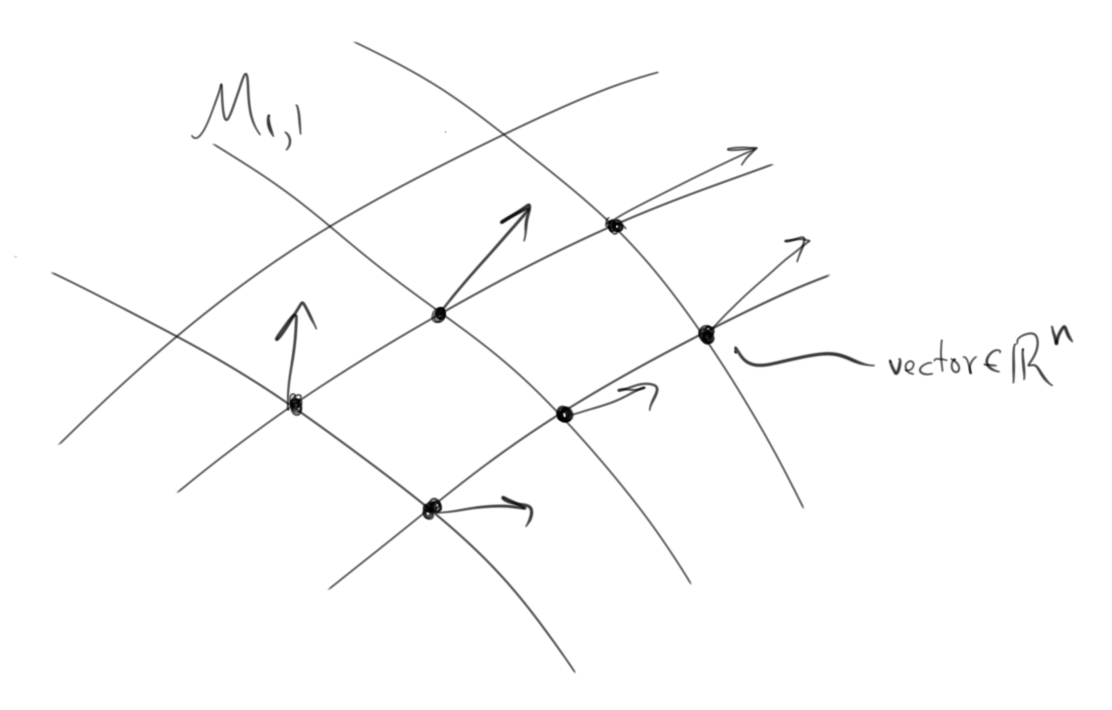
\includegraphics[scale=0.25]{images/vectorfield.png}
		\caption{Sketch of the vector field $\rho = \mathbb{R}^n$ over the Minkowski space $\mathcal{M}_{1,1}$.}
		\label{fig:fig1}
	\end{figure}
\item $\rho = \mathcal{S}^2$;  \textbf{vector field on the surface of a sphere};  $\sigma$-model, quantum magnets
\item $\rho = \mathcal{S}^1 \times \mathcal{S}^1$; \textbf{vector field on a torus}; Chern-Simons theory, Lie groups
\end{itemize}

\noindent Note that when our target space is the $N$-dimensional real vector field $\mathbb{R}^N$, the vector field is described as a list $N$ scalar fields $\{\phi_a(x)\}_{a=1}^N$, where $x$ is the coordinate four-vector.

\subsection*{Dynamics of Classical Fields}

\noindent We restrict this to discussion to classical dynamics generated by Lagrangians, obtained via the variational principle applied to th action functional, where the system of scalar fields $\{\phi_a(x)\}_{a=1}^N$, and $a$ labels the particle type (e.g., charge). The action functional $\mathcal{S}$ contains a function of the Langrangian density $\mathscr{L} = \mathscr{L}(\phi_a, \partial_\mu \phi_a)$. The Lagrangian density is actually a function of higher order derivatives of the fields $\phi_a$, but we make the assumption and approximation of first order derivatives, based on observation
\begin{equation}
\mathcal{S}(\Omega) = \int_\Omega d^4 x \,\, \mathscr{L}(\phi_a, \partial_\mu \phi_a). 
\end{equation}

\noindent Where $d^4 x = dx_0 dx_1 dx_2 dx_3$ and $\Omega \subset \mathcal{M}_{1,3}$, as a measurable set, is a region in $(3+1)$-dimensional spacetime. Typically, we consider the spacetime region as the entire Minkowski space $\Omega = \mathcal{M}_{1,3}$. \\

\noindent To extract the equations of motion, we suppose that the action $\mathcal{S}$ is stationary under infinitesimal variations of the component scalar fields $\phi_a(x) \rightarrow \phi_a(x) + \delta \phi_a(x)$, which vanish on the spacetime region boundary, such that $\delta\phi_a(x) = 0$ on $\partial\Omega$.  \\

\noindent Varying the action functional, we obtain $N$ \textit{Euler-Lagrange equations of motion}
\begin{align}
	\delta \mathcal{S} ( \Omega ) &= \int_\Omega d^4 x \,\, \left( \frac{\partial \mathscr{L}}{\partial \phi_a} \delta \phi_a + \frac{\partial \mathscr{L}}{\partial ( \partial_\mu \phi_a )} \delta ( \partial_\mu \phi_a ) \right) \\
	0 &= \int_\Omega d^4 x \,\, \left( \frac{\partial \mathscr{L}}{\partial \phi_a} \delta \phi_a - \frac{\partial}{\partial x^\mu} \left( \frac{\partial \mathscr{L}}{\partial ( \partial_\mu \phi_a )} \right) \right) \delta\phi_a + \int_\Omega d^4 x \,\, \frac{\partial}{\partial x^\mu} \left( \frac{\partial \mathscr{L}}{\partial ( \partial_\mu \phi_a )} \delta \phi_a \right) \\
	0 &= \int_\Omega d^4 x \,\, \left( \frac{\partial \mathscr{L}}{\partial \phi_a} \delta \phi_a - \frac{\partial}{\partial x^\mu} \left( \frac{\partial \mathscr{L}}{\partial ( \partial_\mu \phi_a )} \right) \right) \delta\phi_a + \partial_\mu \mathcal{M}^\mu.
\end{align}

\noindent The last term is a surface term which vanishes on the boundary, since we first demanded that $\delta\phi_a = 0$ vanishes on the boundary, such that $\partial_\mu \mathcal{M}^\mu = 0$ on $\partial\Omega$. \\

\noindent Since $\mathcal{S}(\Omega)$ is stationary with respect to all variations of the fields $\delta\phi_a$ and admissable spacetime regions $\Omega$, the integrand of the remaining term must also vanish $\forall \, a = 1, 2,... \, , N$, and we obtain the $N$ Euler-Lagrange equations of motion
\begin{equation}
-\frac{\partial \mathscr{L}}{\partial \phi_a} + \frac{\partial}{\partial x^\mu} \left( \frac{\partial \mathscr{L}}{\partial (\partial_\mu \phi_a)} \right) = 0.
\end{equation}

\noindent So, with equations of motion in hand, gotten by whatever means, they can be encoded in the Langrangian density, and then recovered via the Euler-Lagrange equations of motion. This allows us to discover equations of motion with certain properties, such as being symmetric under the Poincar\'e transformations, by designing Lagrangian densities, which are scalars under these symmetry transformations, apply Euler-Lagrange "recipe", and get the equations of motion, which are guaranteed to be symmetric under the chosen transformations. This benefit of the action principle makes it easy to design equations of motion with certain symmetries. \\

\subsection*{Example: Klein-Gordon field}

Consider the Langrangian density 
\begin{align}
\mathscr{L} &= \frac{1}{2}\dot{\phi}^2 - \frac{1}{2}(\nabla\phi)^2 - \frac{1}{2}m^2\phi^2 \\
&= \frac{1}{2}(\partial_\mu \phi)^2 - \frac{1}{2}m^2\phi^2
\end{align}

\noindent Where $\dot{\phi} = \partial_0 \phi$ is the time derivative of the field, and $(\nabla\phi)_j = \partial_j\phi$ for $j=1, 2, 3$ are the $x$, $y$, $z$ spatial components of the field derivatives. \\

\noindent Apply the Euler-Lagrange equations of motion to obtain the dynamics of the Klein-Gordon field
\begin{align}
-\frac{\partial \mathscr{L}}{\partial \phi_a} + \frac{\partial}{\partial x^\mu} \left( \frac{\partial \mathscr{L}}{\partial (\partial_\mu \phi_a)} \right) &= 0 \\
\frac{\partial}{\partial x^\mu}(\partial^\mu \phi) -(-m^2 \phi) &= 0 \\
\partial_\mu \partial^\mu \phi + m^2 \phi &=0 \\
\Box \phi + m^2 \phi &= 0
\end{align}

\subsection*{Hamiltonian formalism}

\noindent A better way to guess/build a quantum theory, with the correct calssical limit determined by the Langrangian density, is the \textit{Hamiltonian formalism}, where we calculate conjugate variables and impose canonical (algebraic) commutation relations. \\

\noindent Suppose that $\phi_a(x)$ is a component field's \textit{canonical position}. Then define the \textit{conjugate momentum density} for each field to be 
\begin{equation}
\pi_a(x) = \frac{\partial \mathscr{L}}{\partial \dot{\phi_a}}.
\end{equation}

\noindent In order to computationally study a field, we discretize the space into a regular lattice with spacing $\epsilon$ between each lattice site, since representing a continuous object on a computer would require an infinite amount of data. Discretization yields generalized coordinates, defined by the field itself, of the form $q_j^a(t) = \phi_a(t, x_j), \, j \in \mathbb{Z}$. For example, consider the $1+1$-dimensional Minkowski space $\mathcal{M}_{1,1}$

\begin{figure}[H]
	\centering
	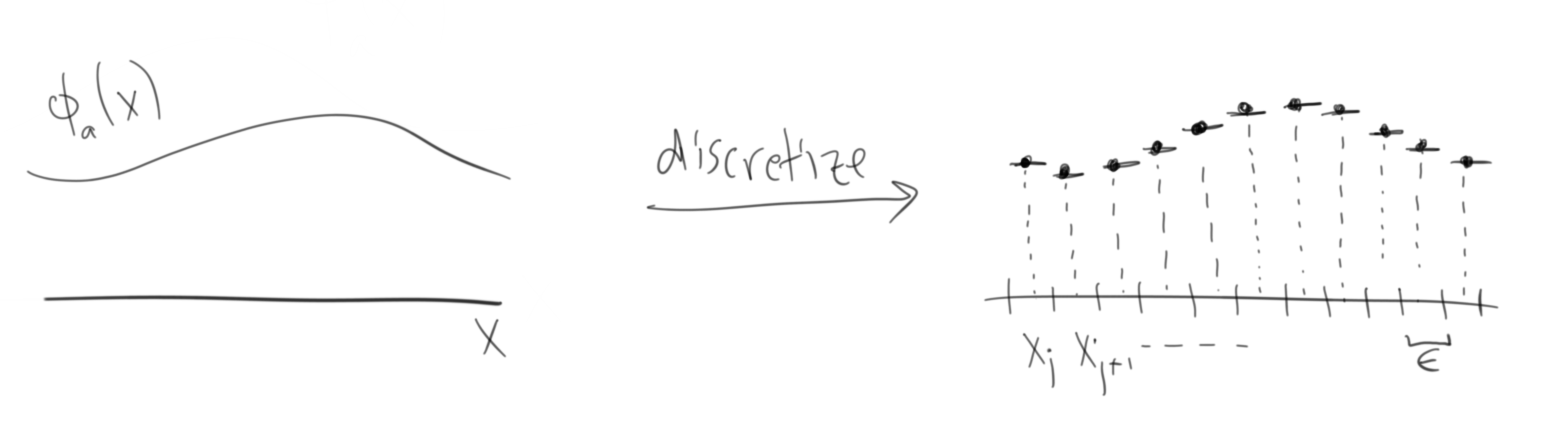
\includegraphics[width=\linewidth]{images/discrete.png}
	\caption{Schematic of field discretization.}
	\label{fig:fig3}
\end{figure}

\noindent To discretize the action functional and apply the variational principle, replace the partial derivatives $\partial_\mu \phi_a(t, x)$, since it is a continuous operation, by applying Taylor's theorem to approximate the spatial component of the field as a finite difference, where $\epsilon$ should be made as small as possible such that the error approximation is minimized
\begin{equation}
\partial_x \phi_a(t, x_j) \cong \frac{\phi_a(t, x_j + \epsilon) - \phi_a(t, x_j)}{\epsilon} = \frac{q^a_{j+1} - q^a_j}{\epsilon}.
\end{equation}

\noindent Leave the temporal component to be continuous
\begin{equation}
\partial_t \phi_a(t, x_j) \cong \dot{q}_j^a . 
\end{equation}

\noindent To obtain the Lagrangian, integrate the density over space, such that only the time dependence is left
\begin{equation}
\int d^3 x \,\, \mathscr{L} (\phi_a, \partial_\mu \phi_a) = L(q_j^a (t), \dot{q}_j^a (t)) = L(t) . 
\end{equation}

\noindent The discrete approximation of the Lagrangian is written as 
\begin{equation}
L(t) \cong \sum_j \delta x_j \mathscr{L}(\phi_a(t, x_j), \partial_\mu \phi_a(t, x_j)). 
\end{equation}

\noindent And the discrete conjugate momenta 
\begin{equation}
p_j^a(t) = \frac{\partial L}{\partial \dot{q}_j^a} = \sum_j \delta x_j \frac{\partial \mathscr{L}}{\partial \dot{q}_j^a} = \sum_j \delta x_j \pi^a(t, x_j).
\end{equation}

\subsubsection*{Simple Example}

\noindent As a simple example, consider the Lagrangian density 
\begin{align}
\mathscr{L} &= \frac{1}{2} (\partial_\mu \phi \partial^\mu \phi) \\
&= \frac{1}{2}(\partial_t \phi)^2 - \frac{1}{2} (\partial_x \phi)^2 .
\end{align}

\noindent (RECHECK) Integrate over space $d^3 x$ to obtain the Lagrangian, and discretize using the rules defined above
\begin{equation}
L(t) = \frac{1}{2} \sum_{j=-\infty}^{\infty} \left( \epsilon \left( \frac{d q_j}{d t} \right)^2 - \frac{(q_{j+1} - q_j)}{\epsilon} \right) .
\end{equation}

\noindent Where $\delta x_j = \epsilon$ and $p_j(t) = \epsilon \frac{d q_j}{dt} = \pi(t, x_j) \delta x_j $. 

\noindent As $\epsilon \rightarrow 0$, $q_j(t) \rightarrow \phi(t, x)$ and $p_j(t) \rightarrow \dot{\phi(t, x)}$

\subsubsection*{Hamiltonian Density}

\noindent For the discrete approximation, the Hamiltonian $H$, obtained by integrating the Hamiltonian density $\mathscr{H}$ of space $d^3 x$, is written as 
\begin{equation}
H = \sum_j p_j^a \dot{q}_j^a - L = \sum_j \delta x_j ( \pi_a(t, x_j) \dot{\phi}_a(t, x_j) - \mathcal{L}_j )
\end{equation}

\noindent In the limit as $\epsilon \rightarrow 0$, the Hamiltonian density is 
\begin{equation}
\mathscr{H}(t, x) = \pi_a(t, x) \dot{\phi}_a(t, x) - \mathscr{L} \left( \phi_a(t, x), \partial_\mu \phi_a(t,x) \right)
\end{equation}

\noindent The Hamiltonian density for the Klein-Gordon field is, dropping the field index and spacetime dependencies from the expression, 
\begin{equation}
\mathscr{H} = \frac{1}{2}\pi^2 + \frac{1}{2}(\nabla \phi)^2 + \frac{1}{2} m^2 \phi^2
\end{equation}